% =============================================================================
% Section 7: Practical Guidelines
% =============================================================================

\subsection{Using the Model}

The simplest approach is to use the \cityseer{} library's adaptive sampling functions, which implement the model automatically (see Section~\ref{sec:cityseer_impl}). For practitioners implementing sampling in other frameworks, the model can be applied manually in three steps:

\begin{enumerate}
\item \textbf{Estimate reach}: For each analysis distance $d$, estimate the mean number of nodes within distance $d$. This can be obtained from a pilot computation on a sample of source nodes, or estimated from network density.

\item \textbf{Compute sampling probability}: Apply the model:
\begin{align}
\effn &= \max\left( \kProp \cdot \sqrt{r}, \minEffN \right) \\
p &= \min\left(1, \frac{\effn}{r}\right)
\end{align}

\item \textbf{Run sampled computation}: Compute centrality from a random subset of sources with probability $p$, then scale results by $1/p$.
\end{enumerate}

\subsection{Quick Reference}

Figure~\ref{fig:guide} provides visual lookup charts for common scenarios.

\begin{figure}[H]
\centering
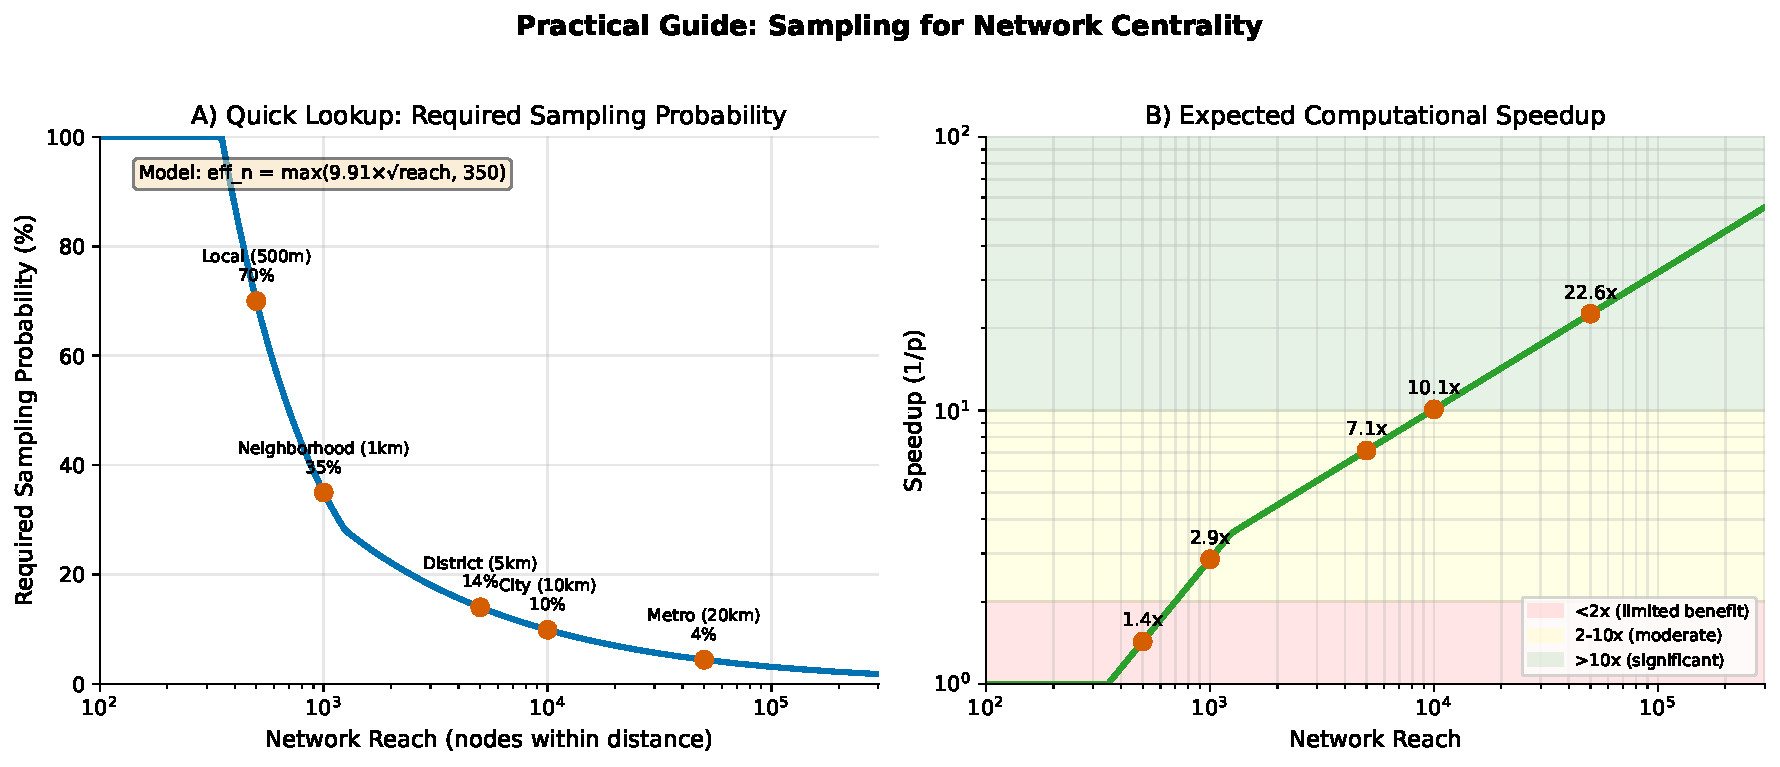
\includegraphics[width=\textwidth]{figures/fig7_practical_guide.pdf}
\caption{\textbf{Practical guidance.} (A) Required sampling probability by network reach, with common urban scenarios annotated. (B) Expected computational speedup.}
\label{fig:guide}
\end{figure}

Table~\ref{tab:lookup} provides a numerical lookup for representative reach values.

\begin{table}[htbp]
\centering
\caption{Practical Sampling Lookup Table}
\label{tab:lookup}
\begin{tabular}{rrrrl}
\toprule
\textbf{Reach} & \textbf{eff\_n} & \textbf{$p$ (\%)} & \textbf{Speedup} & \textbf{Typical Scenario} \\
\midrule
100 & 350 & 100.0 & 1.0$\times$ & Very local \\
200 & 350 & 100.0 & 1.0$\times$ & Local \\
500 & 350 & 70.0 & 1.4$\times$ & 500m walking \\
1,000 & 449 & 44.9 & 2.2$\times$ & Neighborhood \\
2,000 & 635 & 31.8 & 3.1$\times$ & District \\
5,000 & 1005 & 20.1 & 5.0$\times$ & 5km cycling \\
10,000 & 1421 & 14.2 & 7.0$\times$ & City \\
20,000 & 2010 & 10.0 & 10.0$\times$ & Metro area \\
50,000 & 3177 & 6.4 & 15.7$\times$ & Regional \\
100,000 & 4494 & 4.5 & 22.3$\times$ & Large regional \\
\bottomrule
\end{tabular}

\vspace{0.5em}
\footnotesize
\textbf{Usage:} Find your network reach (nodes within analysis distance), read off the required sampling probability.\\
\textbf{Model:} $n_{\mathrm{eff}} = \max(14.21 \cdot \sqrt{r}, 350)$, $p = n_{\mathrm{eff}} / r$.
\end{table}


\subsection{Rules of Thumb}

For practitioners who need quick guidance without computing exact model predictions:

\begin{itemize}
\item \textbf{Small networks or short distances} (reach $< \crossoverReach$): Use full computation ($p = 1.0$). The overhead of sampling setup outweighs any savings.

\item \textbf{Medium networks} (reach 1,000--10,000): Sample 10--30\% of sources. Expect 3--10$\times$ speedup.

\item \textbf{Large networks or long distances} (reach $> 10,000$): Sample 5--15\% of sources. Expect 7--20$\times$ speedup.

\item \textbf{Very large networks} (reach $> 50,000$): Sample 2--5\% of sources. Expect 20--50$\times$ speedup.
\end{itemize}

\subsection{When to Sample More}

The model targets $\rho \geq \targetRho$ with high probability. For applications requiring higher accuracy:

\begin{itemize}
\item \textbf{Higher confidence}: Increase $\effn$ by a factor of 1.5--2$\times$ to achieve $\rho \geq \glaMinRho$.
\item \textbf{Lower variance}: Run 2--3 replications with different random seeds and average results.
\item \textbf{Absolute accuracy}: For applications requiring accurate magnitudes (not just rankings), use higher $\effn$ or consider the scale correction factor from sampled/true ratios.
\end{itemize}

\subsection{When Not to Sample}

Sampling is not appropriate in all cases:

\begin{itemize}
\item \textbf{Very short distances} (reach $< 100$): Full computation is fast; sampling adds overhead with minimal benefit.
\item \textbf{Single-node analysis}: When centrality is needed for specific nodes rather than the full network, targeted computation is more efficient.
\item \textbf{Exact values required}: When application requires exact centrality values (not approximations), sampling is unsuitable.
\item \textbf{Very small networks}: For networks under 1,000 nodes, full computation is typically fast enough that sampling complexity is not justified.
\end{itemize}

\subsection{Implementation in \cityseer{}}
\label{sec:cityseer_impl}

The sampling model is implemented in the \cityseer{} Python library (version 4.23+). Dedicated adaptive functions automatically probe reachability and compute optimal sampling probabilities:

\begin{verbatim}
from cityseer.metrics import networks

# Adaptive per-distance sampling (recommended)
gdf = networks.node_centrality_shortest_adaptive(
    network_structure,
    nodes_gdf,
    distances=[500, 1000, 2000, 5000, 10000],
    compute_closeness=True,
    compute_betweenness=True,
    target_rho=0.95  # Target accuracy
)
\end{verbatim}

The adaptive function automatically:
\begin{enumerate}
\item Probes reachability at each distance via spatially-distributed samples
\item Applies the fitted model to compute sampling probability per distance
\item Runs centrality computation with distance-specific sampling
\item Scales results and returns estimates preserving ranking accuracy
\end{enumerate}

For manual control, a fixed sampling probability can be specified:
\begin{verbatim}
# Manual uniform sampling
gdf = networks.node_centrality_shortest(
    network_structure,
    nodes_gdf,
    distances=[5000],
    sample_probability=0.2  # 20% sampling at all distances
)
\end{verbatim}

\subsubsection{Helper Functions}

The \texttt{cityseer.config} module provides utility functions for custom sampling workflows:

\begin{description}
\item[\texttt{compute\_required\_p(reach)}] Returns the sampling probability from the fitted model. Implements $p = \min(1, \effn / r)$ where $\effn = \max(k \cdot \sqrt{r}, \text{min\_eff\_n})$.

\item[\texttt{probe\_reachability(network, distances)}] Estimates mean reach per distance using spatially-distributed probes. Useful for planning sampling before committing to full computation.

\item[\texttt{spatial\_sample(network, n)}] Returns $n$ node indices distributed across the network using grid stratification, ensuring representative spatial coverage.
\end{description}

Example workflow for custom implementations:
\begin{verbatim}
from cityseer.config import compute_required_p, probe_reachability

# Estimate reach at each distance
reach_estimates = probe_reachability(network, [5000, 10000, 20000])

# Compute required p for each distance
for dist, reach in reach_estimates.items():
    p = compute_required_p(reach)
    print(f"{dist}m: reach={reach:.0f}, p={p:.1%}")
\end{verbatim}
